\subsubsection{Procedure}
\subsubsubsection{Formalizzazione dei documenti}
Un documento può trovarsi in tre stadi diversi:
\begin{itemize}
\item \textbf{In lavorazione:} quando necessita di modifiche, da appena creato e per tutto il periodo necessario alla sua realizzazione;
\item \textbf{Da verificare:} dopo il termine della sua realizzazione, quando viene preso in consegna dai \rVs, che avranno il compito di rilevare e correggere eventuali errori o imprecisioni;
\item \textbf{Approvato:} dopo l'approvazione del \rRP, che avviene dopo il termine della fase di verifica.
\end{itemize}
Ogni documento ripeterà questo suo ciclo interno ad ogni avanzamento di fase, cioè ogni volta che avverrà un aumento dell'indice di versione più significativo.
Tale procedura di formalizzazione viene riassunta nel diagramma di attività indicato in \customRef{fig:formalizzazioneDocumenti}{figura}.
\begin{figure}[H]
\centering
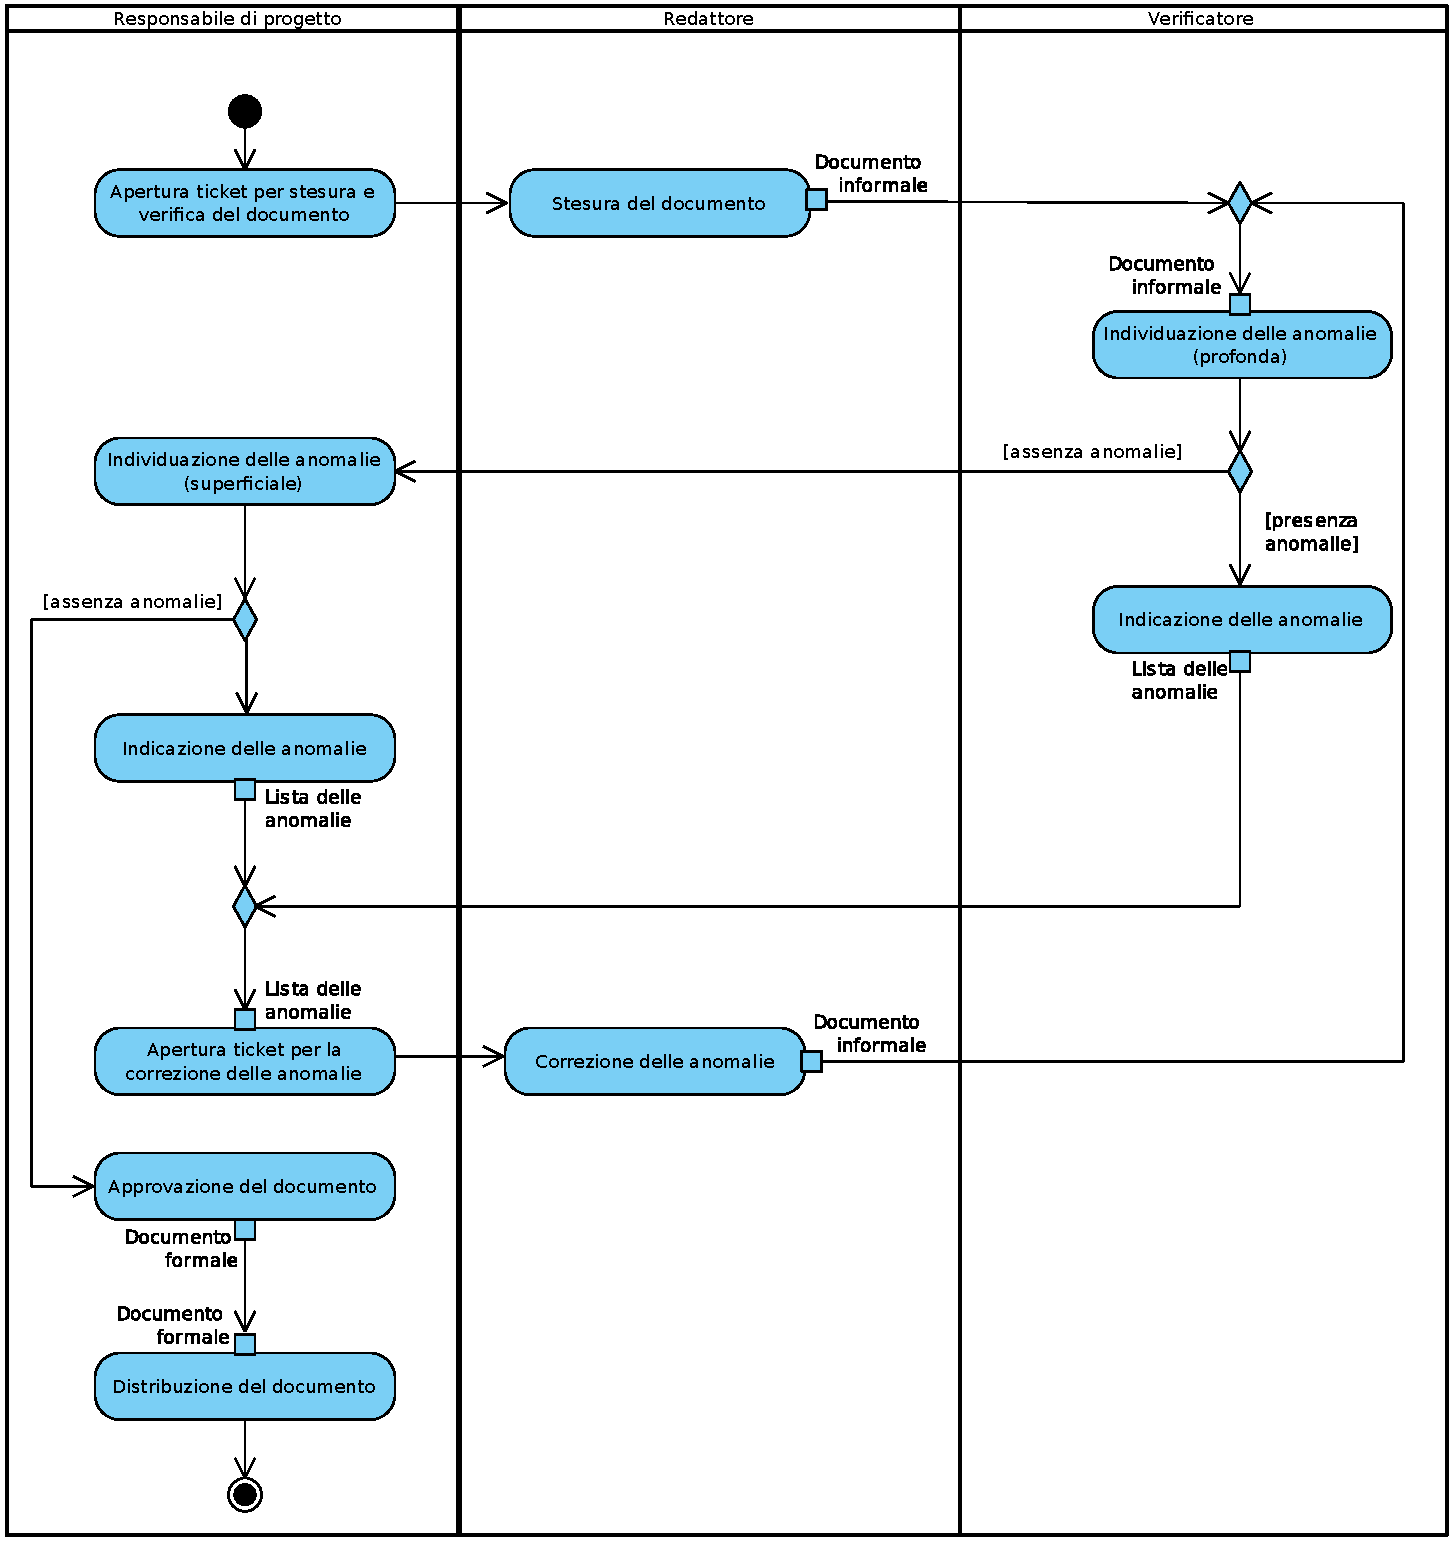
\includegraphics[width=14cm]{../immagini/formalizzazioneDocumenti.pdf}
\caption{Diagramma di attività - formalizzazione di un documento}
\label{fig:formalizzazioneDocumenti}
\end{figure}
